\part{Debugging}
\frame{\partpage}

\begin{frame}{OpenGL Error States}
	\begin{itemize}
		\pause\item \lstinline{glGetError()} queries behind-the-scenes error flags to check state.
		\pause\item Possible \lstinline{glEnum} error codes for each function are listed in the documentation, e.g. for glBindTexture:
	\end{itemize}
	\begin{figure}[h!]
		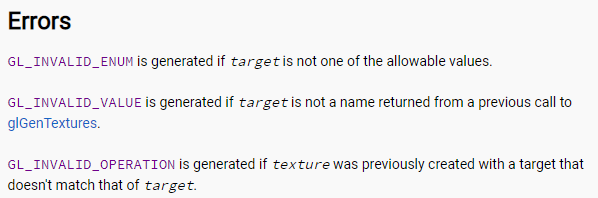
\includegraphics[width=0.8\textwidth]{glerrors}
	\end{figure}
\end{frame}

\begin{frame}[fragile]{Debug Output}
	\begin{itemize}
		\pause\item Extension made core feature from v4.3
		\pause\item Includes information about the cause and severity.
	\end{itemize}
	\pause\begin{lstlisting}
SDL_GL_SetAttribute(SDL_GL_CONTEXT_FLAGS,
		SDL_GL_CONTEXT_DEBUG_FLAG);	// Set up debug context
glEnable(GL_DEBUG_OUTPUT);
glEnable(GL_DEBUG_OUTPUT_SYNCHRONOUS);
glDebugMessageCallback(debugMessage, NULL);
glDebugMessageControl(GL_DONT_CARE, GL_DONT_CARE,
		GL_DONT_CARE, 0, NULL, GL_TRUE);	// Filter errors

// Callback
void APIENTRY debugMessage(GLenum source, GLenum type,
	GLuint id, GLenum severity, GLsizei length,
	const GLchar *message, const void *userParam) {
	// Do something with the error info
	// (print, write to file etc.)
}
	\end{lstlisting}
\end{frame}

\begin{frame}{Debugging Shaders}
	\begin{itemize}
		\pause\item Basic information from \textbf{compilation error reports}.
		\pause\item OpenGL GLSL \textbf{reference compiler} tests shader code against OpenGL specification.
		\pause\item Can use \textbf{colour channels} to display values.
		\pause\item Display \textbf{framebuffer contents} in the corner of the screen (similar to post-processing setup).
		\pause\item More detailed inspection requires using a \textbf{3rd party tool} (depending on GPU vendor etc.).
	\end{itemize}
\end{frame}